\clearpage
\VerdierPhysicalPageAnchor{0089}%
\VerdierSemanticAnchor{ch1-3-2-5-composite-zero-conclusion}
因此它为零。由映射锥函子的伴随性质 (3.1.3)，存在唯一态射：

\VerdierSemanticAnchor{ch1-3-2-5-eq2}
\begin{equation}
  J\colon c(p(f))\longrightarrow X[1],
  \tag{3.2.5.2}
\end{equation}

\noindent 使得下图交换：

\VerdierSemanticAnchor{ch1-3-2-5-eq3}
\VerdierSemanticAnchor{ch1-3-2-5-j-comparison-diagram}
\begin{equation}
  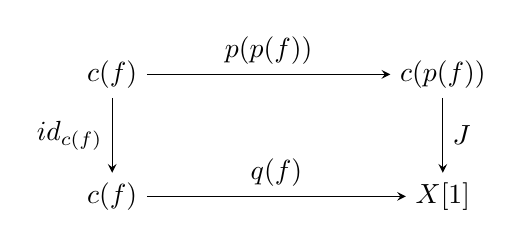
\begin{tikzpicture}[>=stealth,baseline=(current bounding box.center)]
    \node (Cf1) at (0,1.55) {$c(f)$};
    \node (Cpf) at (4.2,1.55) {$c(p(f))$};
    \node (Cf2) at (0,0) {$c(f)$};
    \node (Xs)  at (4.2,0) {$X[1]$};
    \draw[->] (Cf1) -- node[above] {$p(p(f))$} (Cpf);
    \draw[->] (Cf1) -- node[left] {$\operatorname{id}_{c(f)}$} (Cf2);
    \draw[->] (Cpf) -- node[right] {$J$} (Xs);
    \draw[->] (Cf2) -- node[above] {$q(f)$} (Xs);
  \end{tikzpicture}
  \tag{3.2.5.3}
\end{equation}

\noindent 并且 $Ja(p(f))=0$ (3.1.2.4)。

\VerdierSemanticAnchor{ch1-3-2-6}
\noindent\textbf{命题 3.2.6.}\quad
\VerdierSemanticAnchor{ch1-3-2-6-a}
\emph{a) 态射 $J$ 是同伦等价；即它在同伦意义下是同构。}

\VerdierSemanticAnchor{ch1-3-2-6-b}
\emph{b) 下图}

\VerdierSemanticAnchor{ch1-3-2-6-eq1}
\begin{equation}
  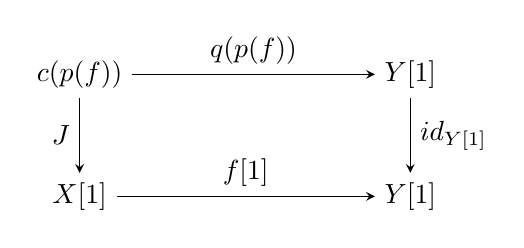
\begin{tikzpicture}[>=stealth,baseline=(current bounding box.center)]
    \node (Cpf) at (0,1.55) {$c(p(f))$};
    \node (Ys1) at (4.2,1.55) {$Y[1]$};
    \node (Xs)  at (0,0) {$X[1]$};
    \node (Ys2) at (4.2,0) {$Y[1]$};
    \draw[->] (Cpf) -- node[above] {$q(p(f))$} (Ys1);
    \draw[->] (Cpf) -- node[left] {$J$} (Xs);
    \draw[->] (Ys1) -- node[right] {$\operatorname{id}_{Y[1]}$} (Ys2);
    \draw[->] (Xs) -- node[above] {$f[1]$} (Ys2);
  \end{tikzpicture}
  \tag{3.2.6.1}
\end{equation}

\noindent\emph{在同伦意义下反交换。}

\VerdierSemanticAnchor{ch1-3-2-7}
\noindent\textbf{3.2.7. 证明。}\quad
\VerdierSemanticAnchor{ch1-3-2-7-h-construction}
首先构造一个态射 $H\colon X[1]\longrightarrow c(p(f))$。
\VerdierSemanticAnchor{ch1-3-2-7-representing-functors}
为此，只需构造这两个对象所表示的两个函子之间的态射。设 $W$ 是
$\operatorname{comp}(C)$ 的一个对象。
\VerdierSemanticAnchor{ch1-3-2-7-pair}
由映射锥函子的伴随性质 (3.1.3)，从 $c(p(f))$ 到 $W$ 的一个态射无非是
一对 $(u,a)$，其中 $u\colon c(f)\longrightarrow W$ 是复形态射，
$a\colon0\rightsquigarrow up(f)$ 是一个同伦。
\VerdierSemanticAnchor{ch1-3-2-7-triple}
再次使用 (3.1.3)，可见从 $c(p(f))$ 到 $W$ 的一个态射就是一个三元组
\begin{equation*}
  \bigl(m\colon Y\longrightarrow W,\quad
  a\colon0\rightsquigarrow m,\quad
  b\colon0\rightsquigarrow mf\bigr).
\end{equation*}
对这个三元组配以下图：

\VerdierSemanticAnchor{ch1-3-2-7-eq1}
\begin{equation}
  \begin{gathered}
    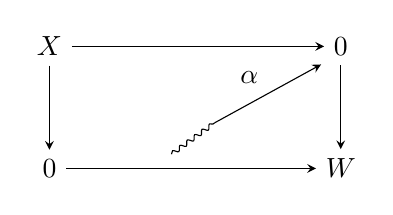
\begin{tikzpicture}[>=stealth,baseline=(current bounding box.center)]
      \node (X)  at (0,1.55) {$X$};
      \node (Z1) at (3.7,1.55) {$0$};
      \node (Z2) at (0,0) {$0$};
      \node (W)  at (3.7,0) {$W$};
      \draw[->] (X) -- (Z1);
      \draw[->] (X) -- (Z2);
      \draw[->] (Z1) -- (W);
      \draw[->] (Z2) -- (W);
      \draw[decorate,decoration={snake,amplitude=0.8pt,segment length=3.3pt}]
        (1.55,0.18) -- (2.10,0.58);
      \draw[->] (2.10,0.58) -- node[above left] {$\alpha$} (3.45,1.32);
    \end{tikzpicture}
    \qquad \alpha=b-a\star f ,
  \end{gathered}
  \tag{3.2.7.1}
\end{equation}
